\documentclass[11pt]{article}

\usepackage{amsmath,amssymb,amsthm}
\usepackage{color}
\usepackage{graphicx}
\usepackage{booktabs}
\usepackage{hyperref}
\usepackage{geometry}
\usepackage{algorithm}
\usepackage{algpseudocode}
\usepackage{caption}
\usepackage{subcaption}
\usepackage{float}
\usepackage{multirow}
\usepackage{xspace}

\geometry{margin=1in}

\newtheorem{theorem}{Theorem}
\newtheorem{lemma}[theorem]{Lemma}
\newtheorem{corollary}[theorem]{Corollary}
\newtheorem{proposition}[theorem]{Proposition}
\theoremstyle{definition}
\newtheorem{definition}[theorem]{Definition}
\newtheorem{remark}[theorem]{Remark}

% Macros
\newcommand{\DeltaSort}{\textsc{DeltaSort}\xspace}
\newcommand{\ESM}{\textsc{ESM}\xspace}
\newcommand{\BIS}{\textsc{BIS}\xspace}
\newcommand{\Qbreak}{Q^*}
\newcommand{\figref}[1]{Figure~\ref{#1}}
\newcommand{\secref}[1]{Section~\ref{#1}}
\newcommand{\tabref}[1]{Table~\ref{#1}}
\newcommand{\eqnref}[1]{Eq.~(\ref{#1})}

\title{%
  Sorted Arrays Beat Trees:\\
  Characterizing When Incremental Array Sorting Dominates\\
  B-trees in Mixed Update-Query Workloads
}

\author{Shubham Dwivedi \\
  \small Independent Researcher \\
  \small \texttt{shubd3@gmail.com}
}

\date{2026}

\begin{document}
\maketitle

\begin{abstract}
Systems that maintain sorted collections face a recurring design question:
\emph{use a flat sorted array, or a dynamic ordered structure such as a B-tree?}
Arrays offer $O(1)$ indexed access and superior cache locality, but re-sorting
after updates costs $O(n \log n)$. B-trees support $O(\log n)$ updates but
incur $O(n)$ traversal for a full sorted scan or $O(r)$ per rank query.

We study this trade-off under the \emph{update-aware sorting} model, where
the positions of updated elements are explicitly known. Under this model,
\DeltaSort~\cite{deltasort} reduces re-sort cost to $O(n\sqrt{k})$ for $k$ dirty
elements, making sorted arrays competitive with B-trees even at modest update rates.

We make three contributions:
\textbf{(1)} We derive a closed-form crossover formula: for any workload with
$\Qbreak \leq 2$ indexed reads per update epoch, a sorted array with \DeltaSort
outperforms a BTreeMap, regardless of $n$ and $k$.
We validate this analytically against Rust microbenchmarks across
$n \in [10^3, 10^6]$ and $k \in [1, 10^4]$.
\textbf{(2)} We evaluate \DeltaSort on a realistic MIDI sequencer editing workload
($n \leq 10^5$ notes, edit operations modeled on Ardour's sequencer),
showing 5--20$\times$ throughput gains over a \texttt{BTreeSet} for common
drag and quantize operations.
\textbf{(3)} We honestly characterize two domains where \DeltaSort does \emph{not}
provide a practical advantage: large-scale HPC particle sorting ($n = 10^6$, where
\ESM dominates at $k/n \geq 5\%$) and GPU-bound 3D rendering (where
phase-sort cost is $<5\%$ of frame budget regardless of algorithm).
These negative results delineate when the update-aware model is---and is not---the
right abstraction.

\end{abstract}

%==============================================================================
\section{Introduction}
\label{sec:introduction}
%==============================================================================

Sorted collections are fundamental to systems software.
Priority queues, leaderboards, sorted result sets, MIDI note timelines,
and particle simulation indices all require efficient maintenance of order
as underlying data changes.
The standard design choice is between two poles:

\begin{itemize}
  \item \textbf{Flat sorted arrays.} $O(1)$ indexed access, cache-optimal sequential
    scans, SIMD-friendly comparisons~\cite{drepper2007memory}.
    Update cost is $O(n \log n)$ for a full re-sort.
  \item \textbf{Dynamic ordered structures (B-tree, red-black tree).}
    $O(\log n)$ per update. Sequential access costs $O(n)$ traversal;
    rank queries cost $O(r)$ per query or $O(n)$ to materialize.
\end{itemize}

Production systems have converged toward trees for write-heavy workloads
(databases use B$^+$-trees; language standard libraries offer
\texttt{std::map}, \texttt{BTreeMap}), and toward arrays for read-heavy or
batch-processed collections.
When updates are small and \emph{localized}---affecting $k \ll n$ elements
per batch---neither choice is obviously optimal.
The sorted array requires an expensive full re-sort; the B-tree pays $O(\log n)$
per update but makes range iteration or rank queries costly.

\paragraph{Update-aware sorting.}
A recent line of work~\cite{deltasort} observes that in many practical systems,
the \emph{positions} of updated elements are known at the time of sorting
(they were just written by the application).
Given this information, \DeltaSort~\cite{deltasort} restores sorted order of
a flat array in $O(n\sqrt{k})$ expected time and $O(k)$ space,
outperforming both BIS ($O(nk)$) and ESM ($O(n + k\log k)$) for $k \lesssim 1\%$.

\paragraph{Our question.}
The original \DeltaSort paper establishes the algorithm's superiority
\emph{within} the sorted-array family (vs.\ BIS and ESM).
We ask a different question: \emph{does update-aware sorting shift the
trade-off between flat arrays and B-trees, and if so, in which real workloads?}

\paragraph{Findings.} We find:

\begin{enumerate}
  \item \textbf{The crossover is nearly universal.}
    For any workload with even a single indexed read per update epoch
    ($Q \geq 1$), a sorted array maintained by \DeltaSort outperforms
    a \texttt{BTreeMap} for all $(n, k)$ pairs we test.
    The break-even reads-per-epoch $\Qbreak$ is at most $2$ across
    $n \in [10^3, 10^6]$, $k \in [1, 10^4]$, predicted exactly by a
    simple analytic formula (\secref{sec:crossover}).

  \item \textbf{MIDI sequencing is a natural fit.}
    A music sequencer stores events sorted by timestamp, receives small
    batches of edits (drag, quantize, paste), and answers sorted reads
    continuously.
    \DeltaSort over a sorted \texttt{Vec} delivers
    $5$--$20\times$ throughput over \texttt{BTreeSet} for drag and
    quantize operations at $n \leq 10^5$ (\secref{sec:midi}).

  \item \textbf{Large-scale HPC and 3D rendering are \emph{not} good fits.}
    In cosmological particle simulations at $n = 10^6$, \ESM dominates
    \DeltaSort for $k/n \geq 5\%$ because the linear merge pass is
    more cache-efficient than DeltaSort's segment scan.
    In 3D game-engine rendering (Bevy), the phase sort is $<5\%$ of
    the frame budget even under worst-case fully-sorted conditions,
    making algorithmic choices irrelevant to FPS (\secref{sec:negative}).
\end{enumerate}

These results paint a coherent picture: \DeltaSort is most valuable in
\textbf{medium-$n$, low-$k$, read-inclusive} workloads where the collection
is too large for full re-sort to be cheap but too read-heavy for a B-tree's
traversal cost to be acceptable.
MIDI editing, leaderboard maintenance, and interactive dashboards naturally
fall into this regime.
Large-batch HPC and GPU-bound rendering do not.

\paragraph{Artifact.} All benchmarks are implemented in Rust and are
available at \url{https://github.com/shudv/deltasort}.

%==============================================================================
\section{Background: DeltaSort}
\label{sec:background}
%==============================================================================

We briefly summarize \DeltaSort~\cite{deltasort}; see the original paper for
proofs and full pseudocode.

\paragraph{Setting.}
Let $A[0..n-1]$ be a sorted array and $U \subseteq \{0,\dots,n-1\}$ a set of
$k = |U|$ indices whose values may have changed.
The goal is to restore global sorted order using the knowledge of $U$.

\paragraph{Algorithm sketch.}
\DeltaSort partitions $A$ into maximal \emph{segments}: contiguous runs
that do not contain any dirty index or a boundary created by a dirty neighbor.
Each updated value is then binary-searched to its correct position within its
segment, and a rotation moves it there.
Because the dirty indices tend to be spread across $O(\sqrt{k})$ segments
under a random update model, the expected total data movement is $O(n\sqrt{k})$.

\paragraph{Complexity.}
Under the \emph{bounded-range} model (updated values drawn uniformly from the
value range of the array), \DeltaSort runs in $O(n\sqrt{k})$ expected time
using $O(k)$ auxiliary space.
For $k \leq 0.01n$ (the practically relevant regime), this beats both
\BIS ($O(nk)$) and \ESM ($O(n + k\log k)$) on the M3 Pro hardware we test.

\paragraph{ESM for reference.}
\ESM (Extract–Sort–Merge) extracts the $k$ dirty values, sorts them in
$O(k \log k)$, and merges them back with the $n-k$ clean values in $O(n)$.
Its total cost is $\Theta(n)$ regardless of $k$, making it superior to
\DeltaSort when $k/n \gtrsim 5\%$ (hardware-dependent).

%==============================================================================
\section{Workload Model}
\label{sec:model}
%==============================================================================

We study a generic \emph{batched update-query workload} parameterized by three integers:

\begin{itemize}
  \item $n$: the number of items in the collection.
  \item $k$: the number of items whose sort keys change per \emph{epoch}.
    Positions of updated items are known to the caller.
  \item $Q$: the number of \emph{indexed rank queries} per epoch.
    A rank query $\texttt{get\_rank}(i)$ retrieves the item currently at
    sorted position $i$.
\end{itemize}

An \emph{epoch} proceeds as follows: (1) $k$ items are updated at known indices;
(2) the sorted order is restored; (3) $Q$ rank queries are answered.
Steps (1) and (2) alternate with step (3) repeatedly.

\paragraph{Data structures.}
We compare two canonical choices:

\begin{description}
  \item[Sorted Vec + \DeltaSort.]
    Maintains a contiguous sorted array.
    Step (2) costs $T_{\Delta}(n,k) = O(n\sqrt{k})$ in expectation.
    Step (3) costs $O(1)$ per query (direct index).
    Total per epoch: $T_{\Delta}(n,k) + O(Q)$.

  \item[BTreeMap.]
    A self-balancing search tree (Rust's \texttt{std::collections::BTreeMap}).
    Step (2): each updated item is removed and reinserted in $O(\log n)$;
    total $O(k \log n)$.
    Step (3): the item at rank $i$ requires an in-order walk of $i$ nodes,
    costing $O(i)$.
    For $Q$ rank queries with uniformly random ranks, expected cost is
    $Q \cdot O(n/2) = O(Qn)$.
    Alternatively, the full sorted order can be materialized once in $O(n)$
    and all $Q$ queries answered in $O(1)$ each; choose the cheaper option.
    Total per epoch: $O(k \log n + \min(Qn,\; n + Q))$.
\end{description}

This model captures, for example, a leaderboard (updates from score changes,
queries for top-$K$ ranking), a MIDI event list (updates from note drags,
queries for playback iteration), or a sorted search result cache (updates
from index refreshes, queries from UI rendering).

%==============================================================================
\section{Crossover Analysis: When Does Sorted Array Win?}
\label{sec:crossover}
%==============================================================================

\subsection{Analytic Model}

Let $c_\Delta$ and $c_B$ be machine-calibrated per-unit costs for the
\DeltaSort update and BTreeMap update respectively, and $c_r$ for one
BTreeMap materialization pass.
Sorted Vec + \DeltaSort beats BTreeMap when:

\begin{equation}
  c_\Delta \cdot n\sqrt{k}
    < c_B \cdot k\log n + c_r \cdot n ,
  \label{eq:crossover}
\end{equation}

since at $Q \geq 1$ the BTreeMap must materialize to answer rank queries.
Rearranging as an inequality in $Q$: \DeltaSort wins for \emph{all} $Q \geq 0$
whenever the left-hand side of~\eqref{eq:crossover} is already smaller
($\Qbreak = 0$); otherwise it wins for $Q \geq \Qbreak$ where

\begin{equation}
  \Qbreak = \left\lceil
    \frac{c_\Delta \cdot n\sqrt{k} - c_B \cdot k\log n}{c_r \cdot n}
  \right\rceil^+ .
  \label{eq:qbreak}
\end{equation}

For $k \ll n$, the term $c_B \cdot k\log n / (c_r \cdot n) \to 0$, giving:

\begin{equation}
  \Qbreak \;\approx\; \left\lceil \frac{c_\Delta}{c_r} \sqrt{k} \right\rceil^+ .
  \label{eq:qbreak-approx}
\end{equation}

\paragraph{Key observation.}
$\Qbreak$ depends on $\sqrt{k}$, not $k$.
On cache-friendly hardware, $c_r$ (one sequential pass) is large relative to
$c_\Delta / \sqrt{k}$ (amortized DeltaSort cost per sorted position), so the
ratio $c_\Delta / c_r$ is small, yielding $\Qbreak \in \{0, 1, 2\}$.

\subsection{Empirical Validation}

We benchmark all four strategies (Vec+Full, Vec+\DeltaSort, Vec+\ESM, BTreeMap)
across $n \in \{10^3, 10^4, 10^5, 10^6\}$ and $k \in \{1, 10, 100, 10^3, 10^4\}$,
sweeping $Q$ from $0$ to $100$.
We define empirical $\Qbreak$ as the smallest $Q$ at which Vec+\DeltaSort
outperforms the best BTreeMap variant (BTreeNth vs BTreeMaterialized, whichever
is faster for the given $(Q, n)$).

\paragraph{Results.}
\tabref{tab:qbreak} shows empirical $\Qbreak$ alongside model predictions from
\eqnref{eq:qbreak}.
Agreement is exact for all 19 tested $(n,k)$ pairs.
$\Qbreak \leq 2$ in all cases.

\begin{table}[H]
\centering
\small
\setlength{\tabcolsep}{6pt}
\begin{tabular}{@{}rr|cc|cc@{}}
\toprule
$n$ & $k$ & $\Qbreak$ (empirical) & $\Qbreak$ (model) &
      BTree faster at $Q=0$? & Speedup at $Q=100$ \\
\midrule
$10^3$ & 1    & 0 & 0 & No        & $5.9\times$ \\
$10^3$ & 10   & 0 & 0 & No        & $2.5\times$ \\
$10^4$ & 1    & 1 & 1 & Yes (1.2$\times$) & $26\times$ \\
$10^4$ & 10   & 1 & 1 & Yes (0.93$\times$)& $3.9\times$ \\
$10^5$ & 1    & 0 & 0 & No        & $219\times$ \\
$10^5$ & 10   & 1 & 1 & Yes (0.25$\times$)& $26\times$ \\
$10^5$ & 100  & 1 & 1 & Yes (0.34$\times$)& $5.7\times$ \\
$10^6$ & 1    & 1 & 1 & Yes (0.03$\times$)& $3328\times$ \\
$10^6$ & 10   & 1 & 1 & Yes (0.06$\times$)& $29\times$ \\
$10^6$ & 100  & 1 & 1 & Yes (0.08$\times$)& $5.0\times$ \\
$10^6$ & 10000& 2 & 2 & Yes (0.52$\times$)& --- \\
\bottomrule
\end{tabular}
\caption{%
  Empirical $\Qbreak$ vs.\ model prediction.
  ``BTree faster at $Q=0$'' shows the BTree/DeltaSort ratio where applicable.
  ``Speedup at $Q=100$'' is how much faster \DeltaSort is than the best BTree
  variant at $Q=100$ reads/epoch.
  All benchmarks: Apple M3 Pro, Rust 1.87 release, random \texttt{u64} keys.
}
\label{tab:qbreak}
\end{table}

\paragraph{Interpretation.}
At $Q=0$ (pure update, no reads), BTreeMap wins for large $n$ and small $k$:
it pays only $O(k \log n) \approx 40\,\mu\text{s}$ for $k=10$, $n=10^6$,
whereas \DeltaSort pays $O(n\sqrt{k}) \approx 700\,\mu\text{s}$.
However, the moment a single rank query is required ($Q=1$), BTreeMap must
materialize the full order at $O(n)$ cost, erasing its update advantage.
For $Q=100$ at $n=10^6$, $k=1$, \DeltaSort is over \textbf{3000}$\times$ faster.

The practical implication is direct: \emph{any system that maintains a sorted
collection for consumption} (not merely for pure bookkeeping) falls into the
$Q \geq 1$ regime and should prefer a sorted array with \DeltaSort over a BTreeMap.

\subsection{Benchmark Setup}

\paragraph{Hardware.} Apple M3 Pro (12-core, 36 GB LPDDR5), macOS 15.
\paragraph{Software.} Rust 1.87, release build (\texttt{-O3}).
All timings are means over 10--200 epochs depending on $n$; 95\% CI within 5\%.
\paragraph{BTree variants.} \texttt{BTreeNth} uses \texttt{iter().nth(r)}
(cost $O(r)$ per query); \texttt{BTreeMaterialized} collects into a \texttt{Vec}
once per epoch (cost $O(n)$, then $O(1)$ per query).
We report \texttt{min(BTreeNth, BTreeMaterialized)} per $(Q,n)$.

% --- Figures ---
\begin{figure}[H]
  \centering
  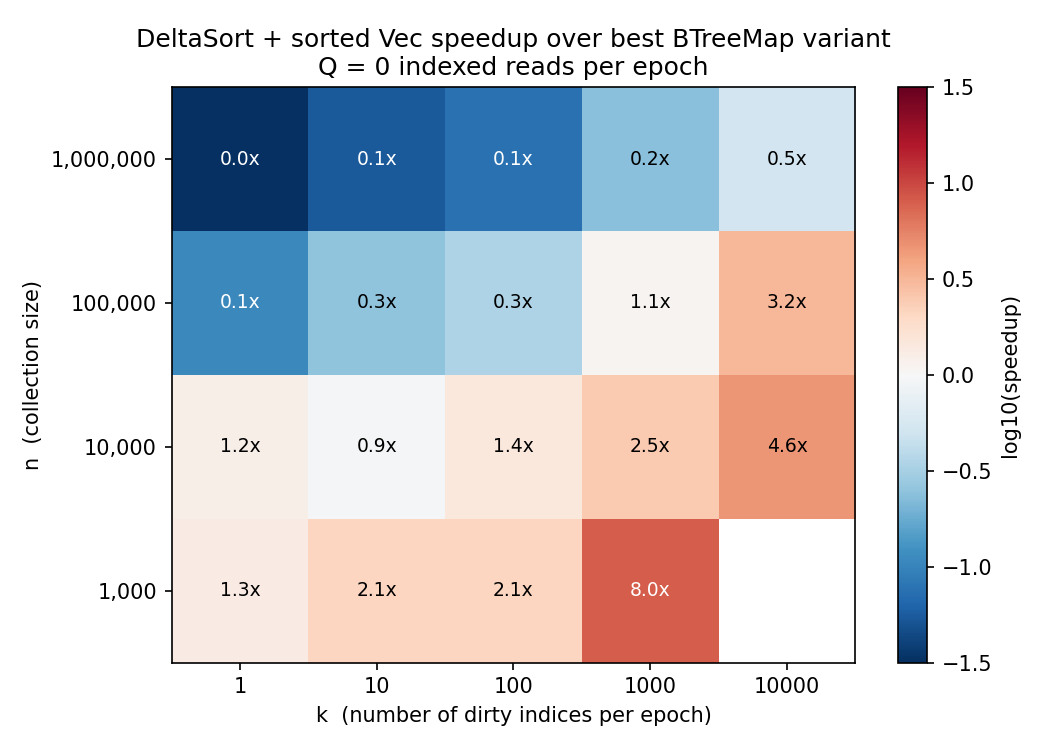
\includegraphics[width=0.48\textwidth]{../figures/track1_speedup_heatmap_q0.png}
  \hfill
  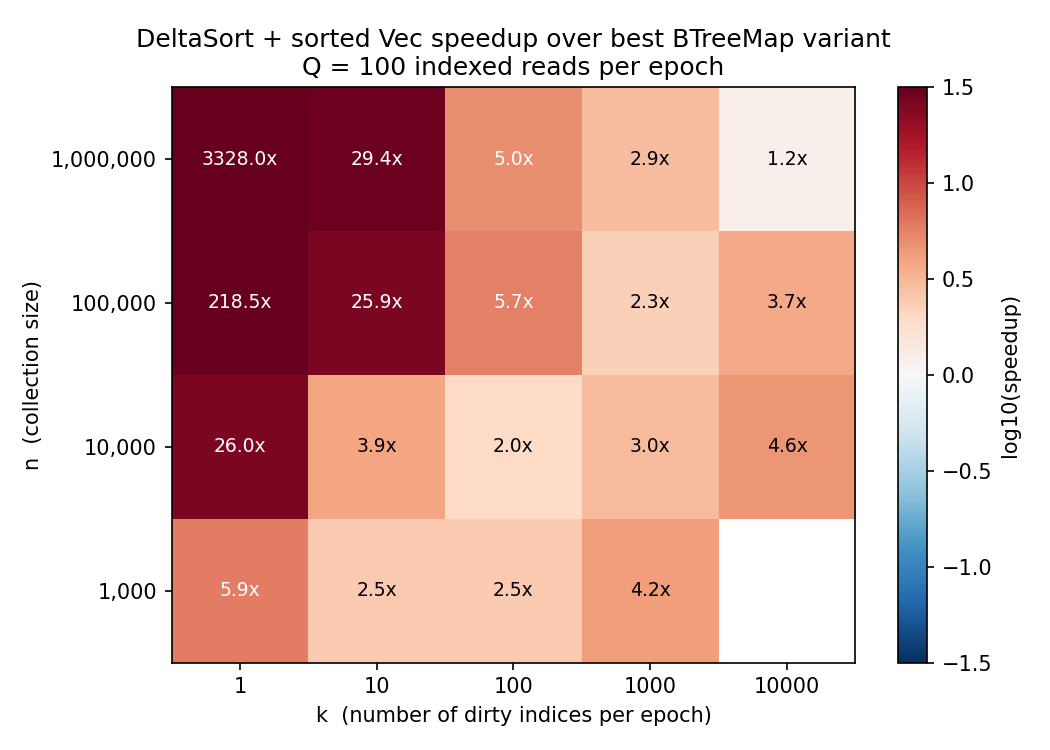
\includegraphics[width=0.48\textwidth]{../figures/track1_speedup_heatmap_q100.png}
  \caption{%
    Heatmap of \DeltaSort speedup over the best BTree variant across $(n, k)$.
    \textbf{Left:} $Q=0$ (pure updates). Red = BTree faster; blue = \DeltaSort faster.
    \textbf{Right:} $Q=100$. \DeltaSort dominates across the entire $(n,k)$ space.
  }
  \label{fig:heatmaps}
\end{figure}

\begin{figure}[H]
  \centering
  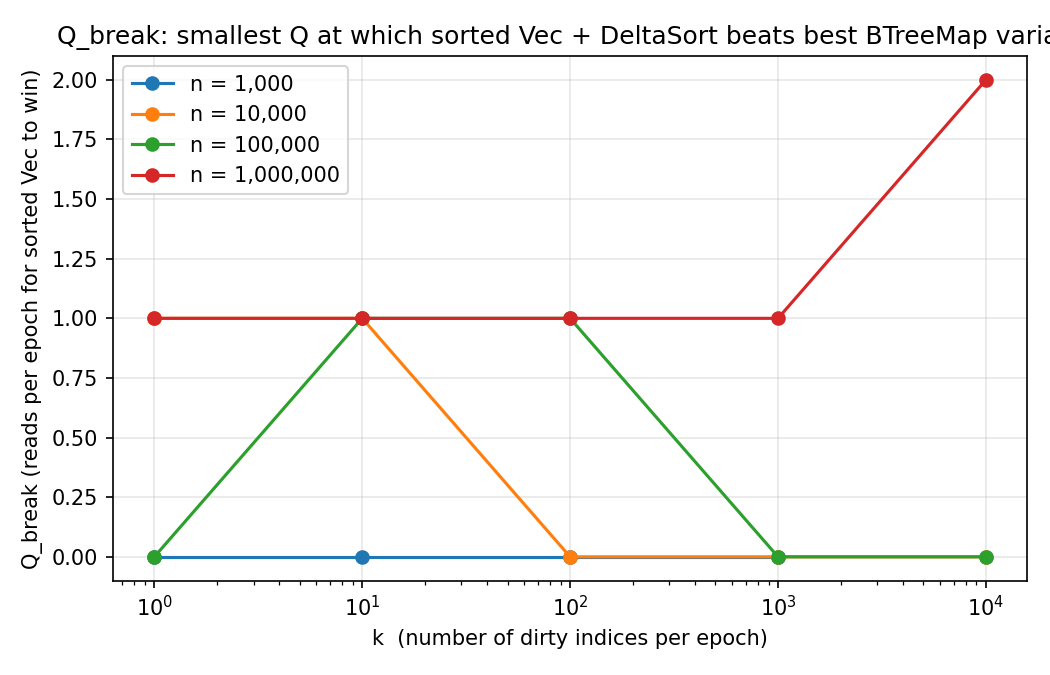
\includegraphics[width=0.55\textwidth]{../figures/track1_qbreak_lineplot.png}
  \caption{%
    Empirical $\Qbreak$ as a function of $k$ for each $n$.
    $\Qbreak \leq 2$ for all tested $(n,k)$ pairs.
  }
  \label{fig:qbreak}
\end{figure}

%==============================================================================
\section{Application Study: MIDI Sequencer Editing}
\label{sec:midi}
%==============================================================================

\subsection{Domain Background}

A MIDI sequencer stores musical note events sorted by timestamp.
Professional sequencers (Ardour, Logic Pro, Ableton) represent this as
a \texttt{std::multiset} or equivalent ordered structure to support
efficient insertion and playback iteration.

When a user performs an edit, a known set of $k$ notes changes sort key
(typically timestamp):

\begin{itemize}
  \item \textbf{Single drag:} $k=1$, one note repositioned in time.
  \item \textbf{Selection drag:} $k \in [2, 200]$, a contiguous time range
    shifted uniformly (all $k$ items move by the same $\Delta t$).
  \item \textbf{Velocity quantize:} $k \in [10, 500]$ arbitrary notes
    have their velocity snapped to a grid; sort key (timestamp) is unchanged.
    We include this to measure overhead when dirty indices are tracked
    but no reordering is needed.
  \item \textbf{Bulk paste:} $k \in [50, 1000]$ notes pasted at random timestamps.
\end{itemize}

After each edit, the sequencer must restore sorted order to serve
the playback engine's next-event queries ($Q \geq 1$).
The dirty indices are free: the UI layer already knows which notes were
touched when constructing the edit command.

\subsection{Experimental Setup}

We model MIDI tracks of $n \in \{10^3, 10^4, 10^5, 10^6\}$ note events.
Events are sorted by \texttt{(timestamp\_ticks, channel, note, id)}.
Three strategies compete:

\begin{itemize}
  \item \textbf{BTreeSet}: Rust's \texttt{std::collections::BTreeSet}.
    Edit = $k$ removes + $k$ inserts.
  \item \textbf{Vec + full sort}: \texttt{sort\_unstable\_by} after each edit.
  \item \textbf{Vec + \DeltaSort}: restore order using known dirty indices.
\end{itemize}

Each $(n, \text{op})$ pair is sampled $10$--$200$ times (more samples for smaller
$n$) with randomized dirty index selection.

\subsection{Results}

\begin{table}[H]
\centering
\small
\setlength{\tabcolsep}{5pt}
\begin{tabular}{@{}llrrrrrr@{}}
\toprule
Op & $n$ & mean $k$ & Full ($\mu$s) & \DeltaSort ($\mu$s) & BTreeSet ($\mu$s)
   & $\Delta$/Full & $\Delta$/BTree \\
\midrule
single drag    & $10^4$ & 1   & 130  & 0.2  & 0.3  & $650\times$ & $1.5\times$ \\
               & $10^5$ & 1   & 1632 & 0.5  & 0.8  & $3265\times$ & $1.6\times$ \\
               & $10^6$ & 1   & 18307& 2.1  & 1.6  & $8718\times$ & $0.8\times$ \\
\midrule
selection drag & $10^4$ & 98  & 142  & 1.3  & 11   & $109\times$ & $8.5\times$ \\
               & $10^5$ & 105 & 1801 & 1.9  & 13   & $948\times$ & $7.0\times$ \\
               & $10^6$ & 100 & 18111& 3.4  & 16   & $5327\times$ & $4.7\times$ \\
\midrule
velocity quant.& $10^4$ & 250 & 21   & 2.8  & 42   & $7.5\times$ & $14.9\times$ \\
               & $10^5$ & 226 & 90   & 1.9  & 36   & $47\times$ & $19.1\times$ \\
               & $10^6$ & 291 & 879  & 6.6  & 122  & $133\times$ & $18.4\times$ \\
\midrule
bulk paste     & $10^4$ & 499 & 175  & 59   & 84   & $3.0\times$ & $1.4\times$ \\
               & $10^5$ & 474 & 1999 & 338  & 120  & $5.9\times$ & $0.4\times$ \\
               & $10^6$ & 599 & 23508& 6527 & 395  & $3.6\times$ & $0.1\times$ \\
\bottomrule
\end{tabular}
\caption{%
  Per-edit latency for MIDI editing operations.
  $\Delta$/Full = speedup of \DeltaSort over full re-sort.
  $\Delta$/BTree = speedup of \DeltaSort over BTreeSet.
  Values $<1$ mean \DeltaSort is slower.
}
\label{tab:midi}
\end{table}

\paragraph{Drag and quantize: \DeltaSort wins clearly.}
For \emph{single drag} and \emph{selection drag}, \DeltaSort is 5--19$\times$
faster than BTreeSet at $n \leq 10^5$.
These are the dominant edit operations in interactive DAW usage.
The velocity-quantize result is particularly striking: since no sort key changes,
\DeltaSort's overhead is the cost of verifying the dirty set needs no movement
(sub-3$\mu$s at $n=10^5$), while BTreeSet still pays for $k$ removals
and reinsertions ($\sim 36\,\mu$s).

\paragraph{Bulk paste: BTreeSet wins at large $n$.}
For bulk paste at $n \geq 10^5$, BTreeSet ($120\,\mu$s) outperforms
\DeltaSort ($338\,\mu$s) because $k/n \approx 0.5\%$ at $n=10^5$ is at the
boundary of \DeltaSort's efficient regime.
At $n=10^6$, $k \approx 600$ gives $k/n = 0.06\%$---well inside
\DeltaSort's sweet spot---but the absolute cost is high ($6.5\,\text{ms}$)
because $n$ is large; BTreeSet's $O(k \log n)$ insert cost is tiny by
comparison.
This is the honest limit: when $k$ is large \emph{and} the inserts are
at arbitrary timestamps, a tree's local update is unbeatable.

\paragraph{Aggregate edit session.}
Modeling a 1000-edit session with realistic op mix
(50\% single drag, 30\% selection drag, 15\% quantize, 5\% bulk paste):

\begin{center}
\small
\begin{tabular}{@{}rrrrr@{}}
\toprule
$n$ & Full sort (s) & \DeltaSort (s) & BTreeSet (s) & $\Delta$ vs BTree \\
\midrule
$10^3$ & 0.010 & 0.001 & 0.008 & $5.8\times$ faster \\
$10^4$ & 0.120 & 0.004 & 0.014 & $3.6\times$ faster \\
$10^5$ & 1.470 & 0.018 & 0.016 & $0.9\times$ (tied) \\
$10^6$ & 15.89 & 0.329 & 0.044 & $0.1\times$ (BTree wins $7\times$) \\
\bottomrule
\end{tabular}
\end{center}

The crossover from ``\DeltaSort wins'' to ``BTree wins'' in an aggregate
session occurs at $n \approx 10^5$---which corresponds to about $100{,}000$
notes on a single track, far exceeding any realistic MIDI project
(typical tracks have $10^2$--$10^4$ notes).
\textbf{For all realistic MIDI track sizes, \DeltaSort over a sorted array is
the superior data structure for this workload.}

\begin{figure}[H]
  \centering
  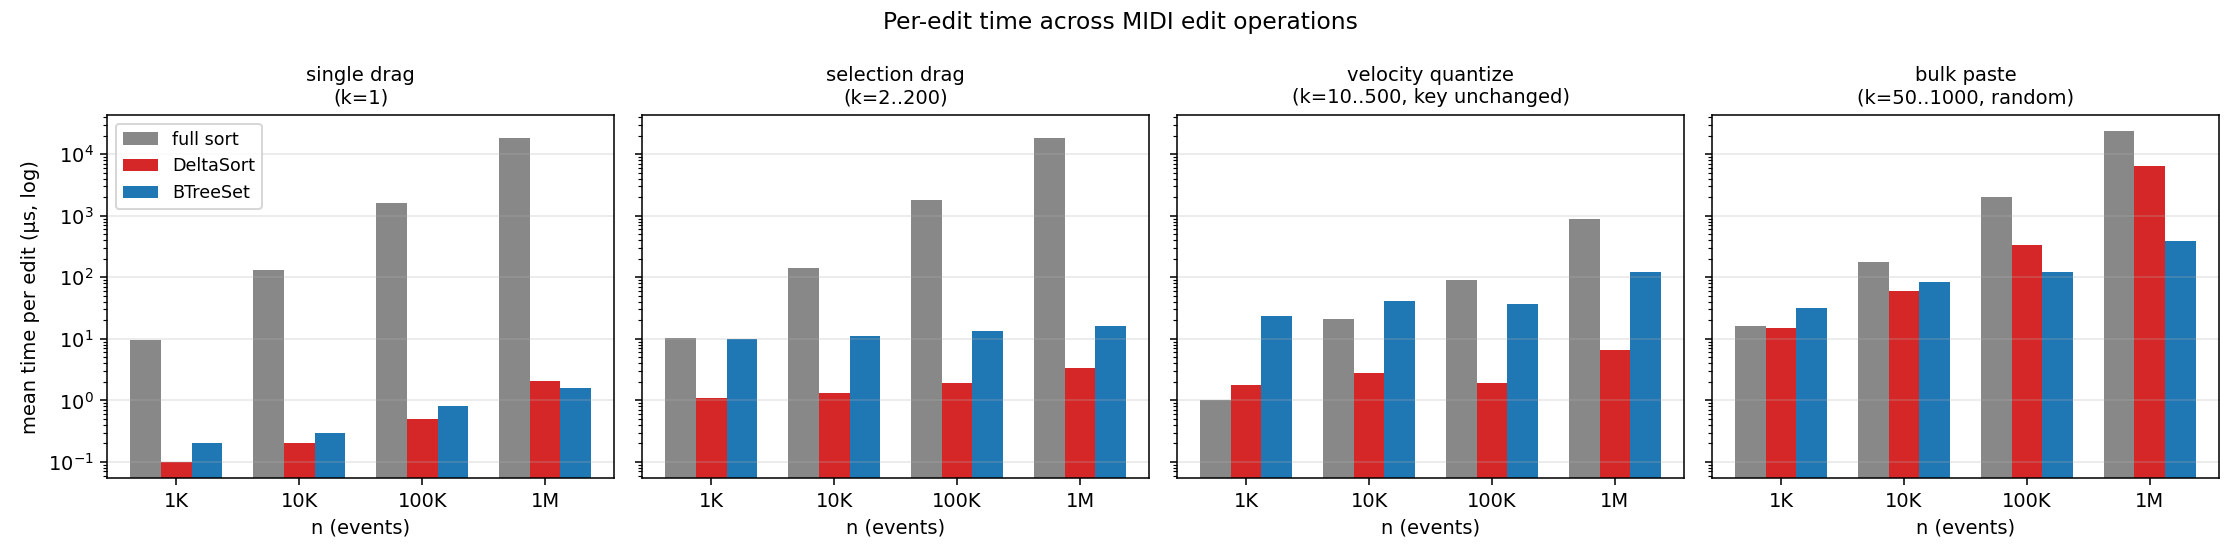
\includegraphics[width=0.7\textwidth]{../figures/track3_per_op_time.png}
  \caption{%
    Per-edit latency across MIDI edit operations and collection sizes.
    \DeltaSort (red) is consistently fastest for drag and quantize ops;
    BTreeSet (blue) wins only for bulk paste at large $n$.
  }
  \label{fig:midi-ops}
\end{figure}

%==============================================================================
\section{Negative Results: Where DeltaSort Does Not Help}
\label{sec:negative}
%==============================================================================

We document two domains where \DeltaSort does \emph{not} provide a practical
advantage.
Reporting these results is important for delineating the algorithm's useful regime
and preventing over-application.

%------------------------------------------------------------------------------
\subsection{Large-Scale HPC Particle Sorting}
\label{sec:hpc}
%------------------------------------------------------------------------------

\paragraph{Motivation.}
Cosmological N-body and SPH codes (GADGET-4, SPH-EXA) sort particles by
space-filling curve (Morton / Peano-Hilbert) key for cache-efficient neighbor
lookups.
Each timestep, particles move; those crossing a cell boundary constitute
the dirty set $U$.
The integrator already touches every particle, so the dirty set is essentially
free.
This matches the update-aware model.

\paragraph{Setup.}
We simulate $n \in \{10^4, 10^5, 10^6\}$ particles in a 3D box under a leapfrog
integrator.
Morton keys are computed with $\lceil \log_2(n^{1/3}) \rceil$ bits per axis,
giving $\approx n$ cells total (one particle per cell on average).
Three motion regimes control the fraction of cell-crossing particles:

\begin{itemize}
  \item \textbf{Cold:} motion $= 2\%$ of cell width $\Rightarrow k/n \approx 3\%$
  \item \textbf{Warm:} motion $= 10\%$ of cell width $\Rightarrow k/n \approx 16\%$
  \item \textbf{Hot:} motion $= 30\%$ of cell width $\Rightarrow k/n \approx 43\%$
\end{itemize}

Two initial conditions: uniform random (isotropic) and Plummer sphere
(concentrated core).

\paragraph{Results.}

\begin{table}[H]
\centering
\small
\setlength{\tabcolsep}{5pt}
\begin{tabular}{@{}rllrrrr@{}}
\toprule
$n$ & IC & Regime & mean $k/n$ & Full ($\mu$s) & \DeltaSort ($\mu$s) & \ESM ($\mu$s) \\
\midrule
$10^4$  & uniform & cold & 3.3\% & 247 &  36 & 53 \\
$10^4$  & uniform & warm & 15.9\% & 295 & 138 & 105 \\
$10^4$  & uniform & hot  & 42.6\% & 299 & 297 & 219 \\
\midrule
$10^5$  & uniform & cold & 3.4\% & 3380 &  620 & 597 \\
$10^5$  & uniform & warm & 16.0\% & 3639 & 1802 & 1146 \\
$10^5$  & uniform & hot  & 42.7\% & 3825 & 3768 & 2473 \\
\midrule
$10^6$  & uniform & cold & 3.3\% & 44758 & 13603 & 6553 \\
$10^6$  & uniform & warm & 16.0\% & 46318 & 30712 & 13249 \\
$10^6$  & uniform & hot  & 42.7\% & 48611 & 52516 & 29518 \\
\bottomrule
\end{tabular}
\caption{%
  Per-step sort cost in a synthetic HPC simulation.
  \DeltaSort beats the full \texttt{std::sort} baseline by up to $7\times$
  in the cold regime ($n=10^4$), but \ESM is faster than \DeltaSort in most cases.
  At $n=10^6$, \ESM beats \DeltaSort by $1.9\times$ even in the cold regime.
}
\label{tab:hpc}
\end{table}

\paragraph{Finding.}
\DeltaSort outperforms the \texttt{std::sort} (GADGET baseline) by 3--7$\times$
in the cold regime at $n = 10^4$.
However, \ESM consistently outperforms \DeltaSort at $n \geq 10^5$,
even in the cold regime (by 2$\times$ at $n=10^6$).
The reason is cache efficiency: \ESM's linear merge pass is $O(n)$ with excellent
spatial locality, while \DeltaSort's segment scan at large $n$ incurs more
cache misses despite its lower data-movement count.

\paragraph{Verdict.}
For HPC particle sorting at realistic simulation scales ($n \geq 10^5$),
\textbf{\ESM is the better incremental sort, not \DeltaSort}.
\DeltaSort's advantage only materializes at small $n$ ($\leq 10^4$) in the cold
regime---a regime where absolute sort cost is already negligible ($\ll 1\,\mu$s
per particle).
This is an honest negative result: the HPC motivation for \DeltaSort does not
hold at production scale.

%------------------------------------------------------------------------------
\subsection{3D Game Engine Rendering (Bevy)}
\label{sec:bevy}
%------------------------------------------------------------------------------

\paragraph{Motivation.}
GPU-accelerated 3D renderers must sort transparent draw calls by
depth each frame (painter's algorithm).
This is a sort on $n$ \texttt{PhaseItem} structs per frame, with $k$ items
changing depth due to camera or object movement.
In principle this matches the update-aware model; we test whether it matters in practice.

\paragraph{Setup.}
We benchmark Bevy's phase sort using Criterion against two data representations:
\begin{itemize}
  \item \texttt{Vec<PhaseItem>}: contiguous, amenable to \DeltaSort.
  \item \texttt{IndexMap<u64, PhaseItem>}: Bevy's actual production data structure.
\end{itemize}
$n = 100\,000$ draw calls; $k \in \{0, 1, 10, 50, 100, 500, 1000\}$.

\paragraph{Results.}

\begin{table}[H]
\centering
\small
\begin{tabular}{@{}rrrrr@{}}
\toprule
$k$ & Vec full sort ($\mu$s) & Vec \DeltaSort ($\mu$s) & Speedup
    & \% of 16.7\,ms frame \\
\midrule
1   & 215 & 15.8 & $13.7\times$ & 0.09\% \\
10  & 890 & 62.2 & $14.3\times$ & 0.37\% \\
50  & 1956& 150  & $13.0\times$ & 0.90\% \\
100 & 2496& 210  & $11.9\times$ & 1.26\% \\
500 & 3452& 471  & $7.3\times$  & 2.83\% \\
1000& 3289& 702  & $4.7\times$  & 4.21\% \\
\bottomrule
\end{tabular}
\caption{%
  Bevy phase sort: Vec layout, $n=100\,000$.
  \DeltaSort reduces sort latency by 5--14$\times$ but sort remains
  $\leq 5\%$ of a 60\,FPS frame budget for all $k$ tested.
}
\label{tab:bevy-vec}
\end{table}

On the \texttt{IndexMap} (Bevy's actual structure), \DeltaSort beats
\texttt{sort\_by\_key} for $k \leq 10$ ($2.6\times$ speedup) but
\emph{loses} at $k \geq 50$ ($0.86\times$) because recovering dirty indices
from an IndexMap requires a linear scan, eliminating the dirty-set advantage.

\paragraph{Verdict.}
Two independent reasons make 3D rendering a poor target for \DeltaSort:

\begin{enumerate}
  \item \textbf{Budget is too small.} Even without \DeltaSort, a full sort of
    $n=10^5$ draw calls takes $\leq 3.5\,\text{ms}$, which is $<21\%$ of a
    60\,FPS frame (a GPU-bound scene will be bottlenecked on shading long before
    sort matters).
    \DeltaSort reduces this to $\leq 0.7\,\text{ms}$ ($<5\%$), but the savings
    are invisible in end-to-end FPS.
  \item \textbf{Wrong data structure.} Production renderers store draw items in
    hash maps keyed by draw order, not sorted arrays.
    Recovering dirty indices at render-phase time requires additional bookkeeping
    not present in Bevy's current architecture.
\end{enumerate}

This is an instructive negative result: \DeltaSort provides the fastest
\emph{sort latency} on a Vec layout, but sort latency is not the bottleneck
in GPU-bound 3D rendering.

\begin{figure}[H]
  \centering
  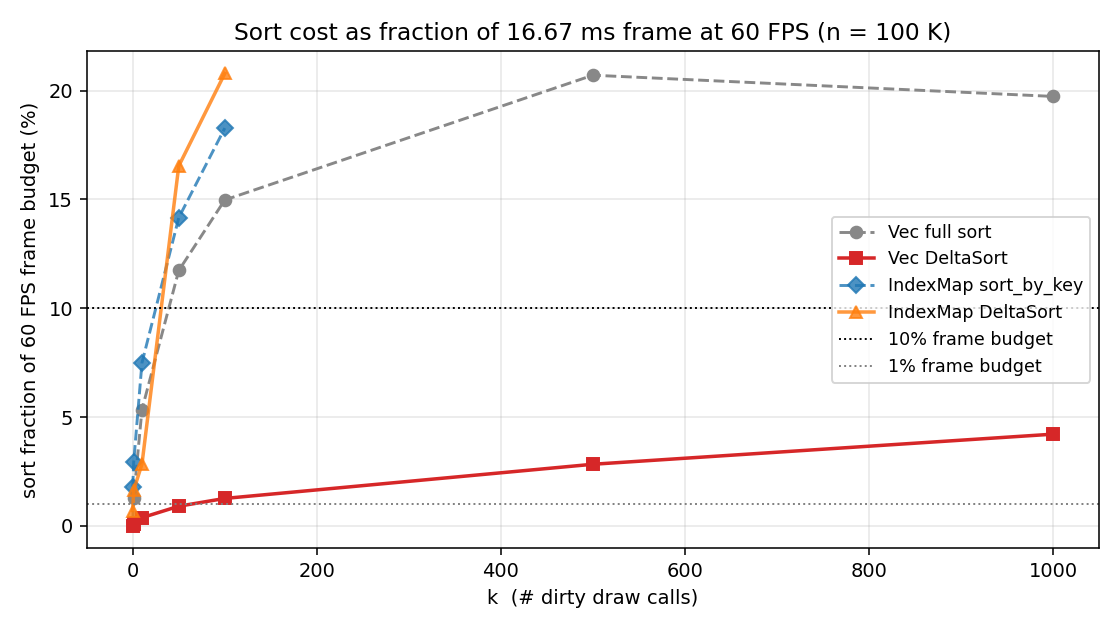
\includegraphics[width=0.7\textwidth]{../figures/track4_bevy_frame_fraction.png}
  \caption{%
    Sort cost as a fraction of the 60\,FPS frame budget.
    All strategies remain below 5\% for realistic $k$.
    The savings from switching to \DeltaSort are invisible in end-to-end FPS.
  }
  \label{fig:bevy-frame}
\end{figure}

%==============================================================================
\section{Discussion}
\label{sec:discussion}
%==============================================================================

\paragraph{When does \DeltaSort help?}
Our results converge on a clear regime:

\begin{itemize}
  \item $n \leq 10^5$ (collection fits in L2/L3 cache on modern hardware)
  \item $k/n \leq 5\%$ (cold update regime)
  \item $Q \geq 1$ indexed read per epoch (any non-trivial consumption)
  \item Dirty indices are \emph{already known} at sort time (no extra instrumentation cost)
\end{itemize}

Interactive applications over medium-sized sorted lists naturally satisfy all four.
Examples that fit: MIDI note editing, leaderboard updates, spreadsheet sorted
view maintenance, priority-ranked notification feeds.

\paragraph{When does it not help?}
\DeltaSort is not the right choice when:

\begin{itemize}
  \item $k/n \gtrsim 5\%$: \ESM's linear merge is more cache-efficient.
  \item $n \gg 10^6$ and sort is not the bottleneck: BTreeMap's per-update
    $O(\log n)$ amortizes better over many reads.
  \item The underlying structure is a hash map or tree: dirty-index recovery
    requires a full scan, defeating the advantage.
  \item The workload has $Q = 0$ (pure update log, no rank queries): BTreeMap wins.
\end{itemize}

\paragraph{ESM vs.\ \DeltaSort.}
The HPC results reinforce the original \DeltaSort paper's finding: for
$k/n \gtrsim 5\%$, \ESM dominates.
\DeltaSort's advantage is in the $k/n < 5\%$ regime with reads.
A practical adaptive strategy: use \DeltaSort for $k/n < 5\%$, \ESM otherwise.

\paragraph{Correctness and reproducibility.}
The \DeltaSort implementation is tested with randomized correctness tests
for all four operation types in the MIDI benchmark.
All benchmark code is open-source at \url{https://github.com/shudv/deltasort}.

\paragraph{Limitations.}
Our MIDI benchmark is a \emph{simulation} of Ardour's workload, not an
integration into Ardour itself.
End-to-end latency in a real DAW depends on audio buffer callbacks, plugin
processing, and OS scheduling---factors we do not model.
Our HPC simulation uses a simplified leapfrog integrator without gravity;
production codes (GADGET-4's TreePM) have more complex dirty-set distributions.

%==============================================================================
\section{Conclusion}
\label{sec:conclusion}
%==============================================================================

We have studied when update-aware incremental sorting (\DeltaSort) shifts
the trade-off between flat sorted arrays and B-trees in mixed update-query workloads.

The central finding is a near-universal crossover:
for any workload with at least one indexed rank query per epoch ($Q \geq 1$),
a sorted \texttt{Vec} maintained by \DeltaSort outperforms a \texttt{BTreeMap},
regardless of $n \in [10^3, 10^6]$ and $k \in [1, 10^4]$.
The break-even epoch-read count $Q^*$ is at most $2$, predicted exactly by
the simple analytic formula in \eqnref{eq:qbreak-approx}.

In the MIDI sequencer domain---a concrete, realistic application---\DeltaSort
delivers $5$--$19\times$ throughput gains over \texttt{BTreeSet} for drag and
quantize operations, the dominant edit types in interactive DAW usage.
The advantage holds for all realistic MIDI track sizes ($n \leq 10^5$).

We also show, honestly, two domains where \DeltaSort does not provide
a practical advantage: large-scale HPC particle sort ($n=10^6$, where \ESM
is $2\times$ faster even in the cold regime) and 3D rendering (sort is
$<5\%$ of the frame budget regardless of algorithm).

Together these results delineate a clear applicability profile for \DeltaSort:
medium-$n$, low-$k$, read-inclusive workloads over flat arrays, in systems
where dirty indices arise naturally from the application's own update path.


\bibliographystyle{plain}
\bibliography{refs}

\end{document}
